
\begin{section}{General User}

    This section describes the shared functionality of all registered users,
    along with the registration, logging in and home page functionality. Note
    that most links on the home page will also be available for logged in users,
    even though this may not always be explicitly mentioned.

    \begin{subsection}{Home Page}

        As this is the first page users see, it's all but obligated to start our
        list of use cases here. Figure \ref{img:index} displays a simple example
        home page. Starting at this home page, the user can complete several
        actions. These are described below.

        \begin{figure}[h]
            \centering
            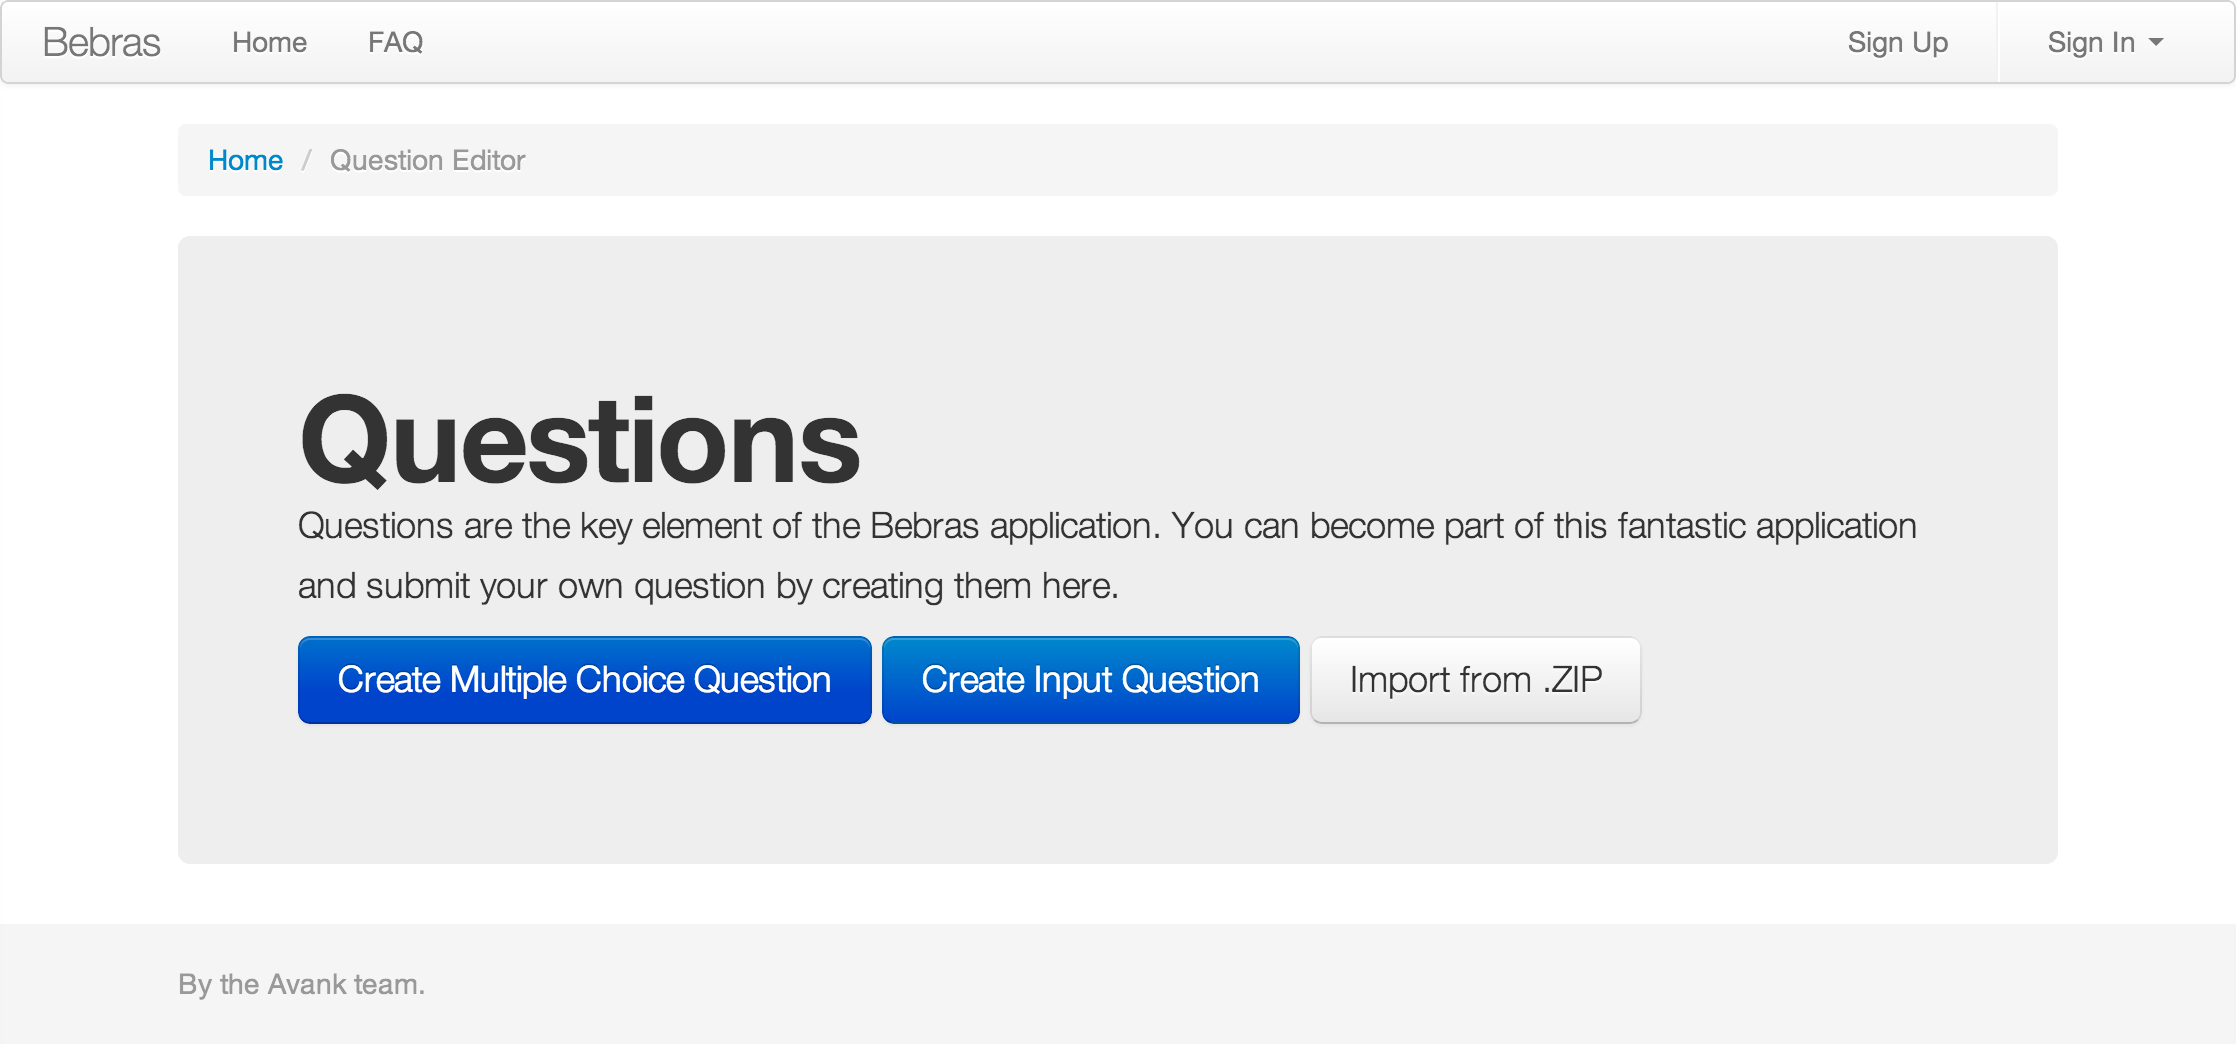
\includegraphics[width=1\textwidth]{index.png}
            \caption{Simplified home page}
            \label{img:index}
        \end{figure}

        \begin{subsubsection}{Log in}
            From the home page, a user can fill in the log in form and hit the
            ``Log in'' button. If the username is valid and the password
            corresponds, the user will be taken to the landing page of this User
            Role. Otherwise, the user is informed of his mistake, so he can try
            again.
        \end{subsubsection}

        \begin{subsubsection}{Register}
            When following the link the user finds on the home page, he is taken
            to a registration page. On this page, the user can fill in
            information about himself, and register.

            There are required fields for the name, gender, birthday and
            password (repeated). The user's preferred language and
            email address are optional. The email address is used when the user
            requests a password reset or contacts an organizer.

            When the information is confirmed by clicking on a ``Register''
            button, the fields are processed. Should the second password not
            match the first, one of the required fields be left empty or one of
            the fields not be conform with its rules (no @ in email, etc...), the
            user is informed and has the chance to refill the incorrect fields.
            Should every form element pass the checks, the user is registered
            succesfully and redirected to the landing page of an Independent
            User.

            Note that special characters in names are supported. We replace them
            with their respective html-escape code to avoid placing the whole
            database in unicode. This conversion is reversed when printing to
            xls files.
        \end{subsubsection}

        \begin{subsubsection}{Register as Teacher}
            An anonymous user can also register himself as a Teacher straight
            away through a webform. In this webform he has to provide either
            the same information as a normal registration or an existing account
            and its password. By providing a telephone number for contact and a
            copy of his teacher's card for verification, he can complete the
            registration. Any organizer can then activate this account when he
            trusts this person to be an actual teacher.
        \end{subsubsection}

        \begin{subsubsection}{Forgot password}
            As we are all forgetful, a user might forget his password. No
            worries, he can follow the ``Forgot password?'' link we will provide
            on the home page. This will take him to a page where he can fill in
            a form with his username and email address. If the user fills in an
            existing username and its corresponding email address, a mail will
            be send there with a new password.

            As there might be users who didn't leave their email address with
            us, the ``Forgot password?'' page will also explain how pupils can
            request a password reset of their teachers. As a final safety net,
            we'll also provide a ``Contact a human'' form, so users other than
            pupils can request the same of an organizer, after convincing him of
            their identity.
        \end{subsubsection}

        \begin{subsubsection}{Go home}
            On the home page is a link to the actual www.Bebras.be site, where
            people can get more information on the organization.
        \end{subsubsection}

        \begin{subsubsection}{Participate in unrestricted contests}
            Straight from the home page, you can also dive into the unrestricted
            quizzes. Just following the link takes you to a list of available
            contests, in which you can participate by clicking on the
            corresponding start buttons.

            When logged in, this page is no longer available. The unrestricted
            contests are listed with the other open contests for your user.
        \end{subsubsection}

        \begin{subsubsection}{Contact a human}
            This link leads to a page containing a form for contacting organizers
            and administrators. Here, the user can select a topic, so mail can
            easily be organized for the readers. A reply-to address must be
            provided.

            Example topics would be ``Teacher Registration'', ``Password
            reset'', ``Question suggestion'', ``Other''.
        \end{subsubsection}

        \begin{subsubsection}{Read Frequently Asked Questions}
            This link on the home page leads you to a page with some frequently
            asked questions. These are indexed and can be searched. The
            organizers can edit these questions and their answers.
        \end{subsubsection}

    \end{subsection}

    \begin{subsection}{Shared Functionality}

        This subsection describes the operations all (registered) users have in
        common. This includes functionality like logging out, changing personal
        information, etc...

        \begin{subsubsection}{Log out}
            Every page except for quiz and contests pages has a log out button.
            Pressing this button logs the user out of the system and brings him
            to the landing page for a not logged in user.
        \end{subsubsection}

        \begin{subsubsection}{Change personal information}
            When any registered user goes to this page using the link on his
            landing page, he can view and change (some of) his personal
            information. An example layout for the page would be Figure
            \ref{img:personal}.

            When the user clicks on any of the ``edit'' links, the corresponding
            data field will turn into a form element, and a simple save button
            needs to be clicked to save the new value. This could look a bit
            like Figure \ref{img:personal_edit}.

            \begin{figure}[h]
                \centering
                \begin{subfigure}{0.7\textwidth}
                    
\includegraphics[width=0.7\textwidth]{personal_u.png}
                    \subcaption{As the page is loaded.}
                    \label{img:personal}
                \end{subfigure}

                \begin{subfigure}{0.7\textwidth}
                    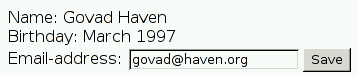
\includegraphics[width=0.7\textwidth]{personal_e.png}
                    \subcaption{When editing the email address.}
                    \label{img:personal_edit}
                \end{subfigure}
                \caption{Simplified layout of the personal page form.}
            \end{figure}
        \end{subsubsection}

        \begin{subsubsection}{View statistics}
            The statistics page is very multifunctional. For each user, this
            page will offer different statistics for different data sets. For
            example, a pupil will be able to see only his own score, with a
            histogram of the other participants' scores. When his teacher looks
            at the same graph, all of his students' scores will be available.
            For an organizer, even more data is readable.

            Apart from several kinds of plots (including but not limited to pie
            charts, histograms and boxplots), you can also download csv files
            with the visible data.

            Now, how do we access this data? We present the user with a few
            options. They can change the data set to any of those within their
            permission:

            \begin{itemize}
                \item \textbf{Independent/Pupil}
                    \begin{itemize}
                        \item His own data.
                        \item The previous and current classes (separate).
                        \item The previous and current schools (separate).
                        \item Everyone's data.
                    \end{itemize}
                \item \textbf{Teacher}
                    \begin{itemize}
                        \item His previous and current classes (separate and
                            together).
                        \item His previous and current schools (separate and
                            together).
                        \item Everyone's data.
                    \end{itemize}
                \item \textbf{Organizer}
                    \begin{itemize}
                        \item Any class (separate and together).
                        \item Any school (separate and together).
                        \item Everyone's data.
                    \end{itemize}
            \end{itemize}

            It's possible to restrict these datasets still. For example, a
            teacher could compare one of his current Ewok classes (e.g., the
            distribution of the scores) with the scores of all of his previous
            Ewok classes.
        \end{subsubsection}

    \end{subsection}

\end{section}


